\chapter{Projekt systemu}
\label{chap:system project}

Poniżej znajduje się projektu systemu będącego aplikacją do planowania trasy dla bezzałogowego statku powietrznego. Zostały tutaj umieszczone cele i przeznaczenie systemu, a także koncepcja rozwiązania. Wykonany projekt obejmuje architekturę systemu, diagram przypadków użycia, diagram klas a także projekt interfejsu użytkownika. 

\section{Cel i przeznaczenie systemu}

Celem systemu jest optymalne wyznaczanie trasy przelotu z uwzględnieniem zadanych parametrów tak, by w możliwie optymalny sposób pokryć teren leśny lub rolny wybrany przez użytkownika. Aby to było możliwe, aplikacja musi wyznaczyć dany obszar na mapie wykorzystując wykrywanie krawędzi.

\section{Koncepcja rozwiązania}



\section{Projekt poszczególnych elementów systemu}

W poniższych sekcjach zostały przedstawione diagramy wraz z opisami ilustrujące działanie systemu oraz jego strukturę. Ponadto, zostanie uzasadniony wybór środowiska oraz wykonanej implementacji.

\subsection{Projekt architektury systemu}

Projekt architektury systemu obejmuje dwie główne części składowe widoczne na schemacie. Ponadto, w projekcie zostało uwzględnione wykorzystanie zewnętrznych API do pobierania danych potrzebnych do działania aplikacji. Jedną z części aplikacji jest frontend, obejmujący implementację interfejsu wykorzystywanego do komunikacji z użytkownikiem i prezentowania wyników działania. Wykorzystane zostało tutaj zewnętrzne API Google Maps, które pozwoli na wybór odpowiedniego obszaru i zaznaczanie punktów przez użytkownika, a także prezentację otrzymanych wyników na rzeczywistym obrazie. Drugą częścią jest backend odpowiedzialny za obsługę żądań oraz wykrywanie obszarów na mapach i planowanie trasy. Ta część systemu będzie wykorzystywała Google Earth Engine API do pobierania zdjęć satelitarnych oraz wykonywania na nich operacji.

\begin{figure}[H]
    \centering
    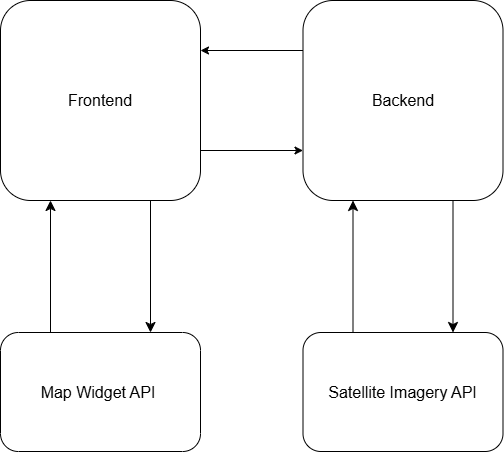
\includegraphics[width=10cm]{images/Architektura_systemu.png}
    \caption{Architektura systemu}
\end{figure}

Na powyższym schemacie widać relacje, jakie zachodzą między poszczególnymi elementami systemu. Frontend będzie wykorzystywał pobrany z API Google Maps komponent mapy, a także będzie wykonywał żądania do backendu w celu zaplanowania trasy dla zadanego terenu. Backend będzie obsługiwał te żądania z wykorzystaniem API Google Earth Engine i zwracał potrzebny wynik do interfejsu w celu zaprezentowania wyników użytkownikowi.

\subsection{Diagram przypadków użycia}

Poniżej został przedstawiony diagram przypadków użycia ilustrujący działanie systemu oraz jego granice, a także opisy każdego z przypadków użycia.

\begin{figure}[H]
    \centering
    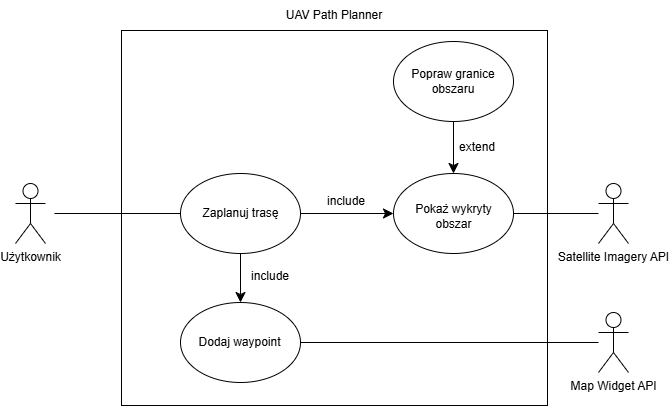
\includegraphics[width=15cm]{images/Diagram_przypadków_użycia.png}
    \caption{Diagram przypadków użycia}
\end{figure}

\hypertarget{plan route}{\textbf{Zaplanuj trasę}} \\*

\textit{Warunki początkowe}

Brak \\*

\textit{Scenariusz interakcji}
\begin{enumerate}
    \item Użytkownik wprowadza prędkość przelotową drona oraz maksymalny czas lotu drona.
    \item Użytkownik wyszukuje na mapie odpowiednie miejsce i wybiera opcję dodania nowego punktu.
    \item Następuje przejście do przypadku użycia \hyperlink{add waypoint}{dodaj waypoint}.
    \item Użytkownik powtarza kroki 2-3 minimum trzy razy.
    \item Użytkownik zatwierdza dodanie wszystkich punktów i następuje przejście do przypadku użycia \hyperlink{show detected area}{pokaż wykryty obszar}.
    \item Użytkownik zatwierdza poprawność wykrytego terenu.
    \item Zostaje wyświetlona zaplanowana trasa na zaznaczonym przez użytkownika terenie.
\end{enumerate}

\vspace{\baselineskip}
\textit{Warunki końcowe}

Brak \\*

\hypertarget{add waypoint}{\textbf{Dodaj waypoint}} \\*

\textit{Warunki początkowe}

Użytkownik wybrał opcję dodania nowego waypointu na mapie \\*

\textit{Scenariusz interakcji}
\begin{enumerate}
    \item Użytkownik nanosi punkt w wybranym miejscu na mapie
    \item W razie potrzeby użytkownik może poprawić położenie punktu
    \item Użytkownik zatwierdza dodanie punktu i następuje powrót do przypadku użycia \hyperlink{plan route}{planowanie trasy}
\end{enumerate}

\vspace{\baselineskip}
\textit{Scenariusz alternatywny}

\begin{adjustwidth}{1.5em}{}
Jeżeli użytkownik zrezygnuje z dodawania punktu może anulować wykonywaną operację w czasie kroków 1-2, a system powróci do \hyperlink{plan route}{poprzedniego przypadku użycia} bez zachowanych zmian.   
\end{adjustwidth}

\vspace{\baselineskip}
\textit{Warunki końcowe}

Pozycja nowego punktu została przechowana w systemie \\*

\hypertarget{show detected area}{\textbf{Pokaż wykryty obszar}} \\*

\textit{Warunki początkowe}

Użytkownik naniósł punkty na mapę i zatwierdził swój wybór \\*

\textit{Scenariusz interakcji}
\begin{enumerate}[label=\arabic*.,ref=\arabic*]
    \item Na ekranie zostaje wyświetlona mapa z naniesionymi na nią punktami oraz wykrytym przez system obszarem.
    \item Użytkownik może obejrzeć cały teren przewijając mapę
    \item Użytkownik dokonuje wyboru:
    \begin{enumerate}[label=\arabic{enumi}.\arabic*.,ref=\arabic{enumi}.\arabic*]
        \item Użytkownik zatwierdza poprawność wykrytego terenu i następuje przejście do przypadku użycia \hyperlink{plan route}{zaplanuj trasę}.
        \item Użytkownik wybiera opcję ręcznej poprawy granic obszaru i następuje przejście do przypadku użycia \hyperlink{change area border}{popraw granice obszaru}.
    \end{enumerate}
\end{enumerate}

\vspace{\baselineskip}
\textit{Warunki końcowe}

Brak \\*

\hypertarget{change area border}{\textbf{Popraw granice obszaru}} \\*

\textit{Warunki początkowe}

Użytkownik wybrał opcję przejścia do poprawy granic wykrytego obszaru \\*

\textit{Scenariusz interakcji}
\begin{enumerate}
    \item Na mapie zostaje wyświetlony wielokąt i jego wierzchołki, które ilustrują wyznaczony teren.
    \item Użytkownik wybiera opcję przeniesienia punktu.
    \item Użytkownik przenosi punkt w nowe, wybrane przez niego miejsce i zatwierdza jego nowe położenie.
    \item Na ekranie pojawia się wykryty teren.
    \item Użytkownik ma możliwość powtórzenia kroków 2-4.
    \item Użytkownik zatwierdza dokonane zmiany i następuje powrót do przypadku użycia \hyperlink{plan route}{planowanie trasy}.
\end{enumerate}

\vspace{\baselineskip}
\textit{Warunki końcowe}

System zapisał zmiany w wykrytym przez niego terenie \\*

\subsection{Diagram klas}

Poniżej znajduje się diagram klas, na którym zostały przedstawione elementy odpowiedzialne za prezentację wyników oraz komunikację z użytkownikiem, a także logikę aplikacji.

\begin{figure}[H]
    \centering
    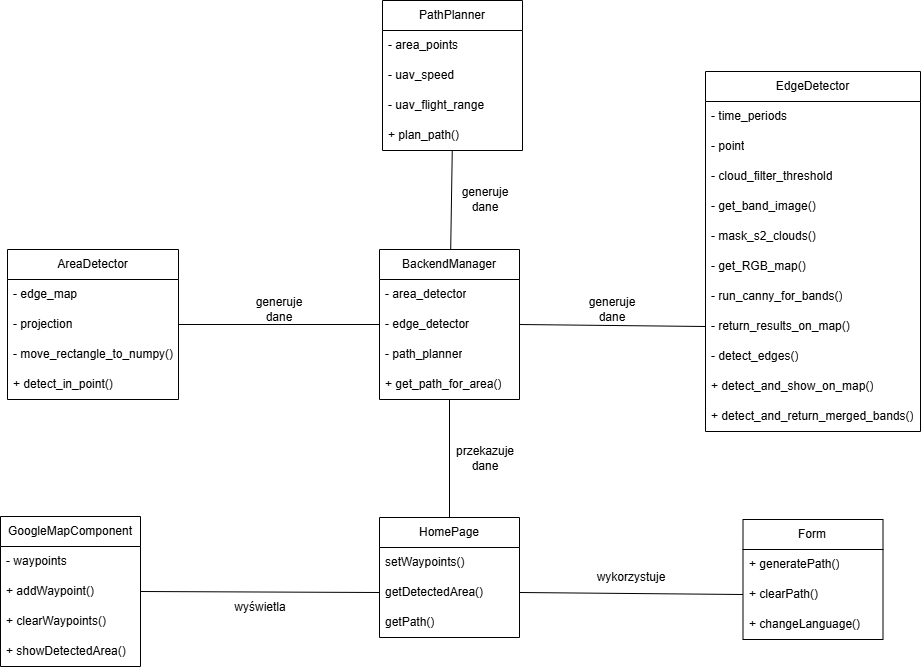
\includegraphics[width=15cm]{images/Diagram_klas.png}
    \caption{Diagram klas}
\end{figure}

Klasa BackendManager jest odpowiedzialna za przepływ sterowania podczas obsługi żądań kierowanych do backendu. Wyniki otrzymane podczas wykrywania obszarów na zdjęciach satelitarnych oraz planowania trasy do wyświetlenia będą zwracane przez tę klasę do interfejsu w celu prezentacji użytkownikowi. Ponadto, dane podane przez użytkownika będą tutaj przetwarzane i przekazywane do odpowiednich części systemu.

Klasa EdgeDetector jest odpowiedzialna za wykrywanie krawędzi na zadanym przez użytkownika obszarze. Będzie przyjmowała punkty podane przez użytkownika i następnie pobierała odpowiednie mapy i wykonywała na nich odpowiednie operacje. Otrzymane wyniki będą zwracane do klasy BackendManager.

Klasa AreaDetector wykrywa obszary na podstawie danych o wykrytych krawędziach na mapie oraz podanych przez użytkownika punktów. Wykryte obszary są przekazywane do BackendManagera w celu prezentacji ich użytkownikowi.

Klasa PathPlanner wytycza trasę przelotu drona na podstawie wykrytego obszaru przekazanego z BackendManagera. Jej wynikiem będą punkty wykrytej trasy, które będą wykorzystywane do prezentowania wyników użytkownikowi na mapie.

Komponent HomePage będzie umożliwiał użytkownikowi kierowanie żądań do backendu i zarządzanie prezentacją otrzymanych wyników podczas wykrywania obszaru i planowania trasy.

Komponent Form będzie odpowiedzialny za pobieranie od użytkownika potrzebnych do zaplanowania trasy danych.

GoogleMapComponent będzie zajmować się pobieraniem od użytkownika punktów wykorzystywanych podczas planowania trasy i wykrywania obszaru, a także prezentacją wyników poszczególnych operacji na mapie.

\subsection{Projekt interfejsu użytkownika}

Po wykonaniu specyfikacji oraz analizy wymagań względem aplikacji został wykonany projekt interfejsu użytkownika z wykorzystaniem narzędzia Figma. Całość została zaprojektowana tak, by obsługa aplikacji była uproszczona i intuicyjna, oraz by prezentowane wyniki były zrozumiałe dla użytkownika.

\begin{figure}[H]
    \centering
    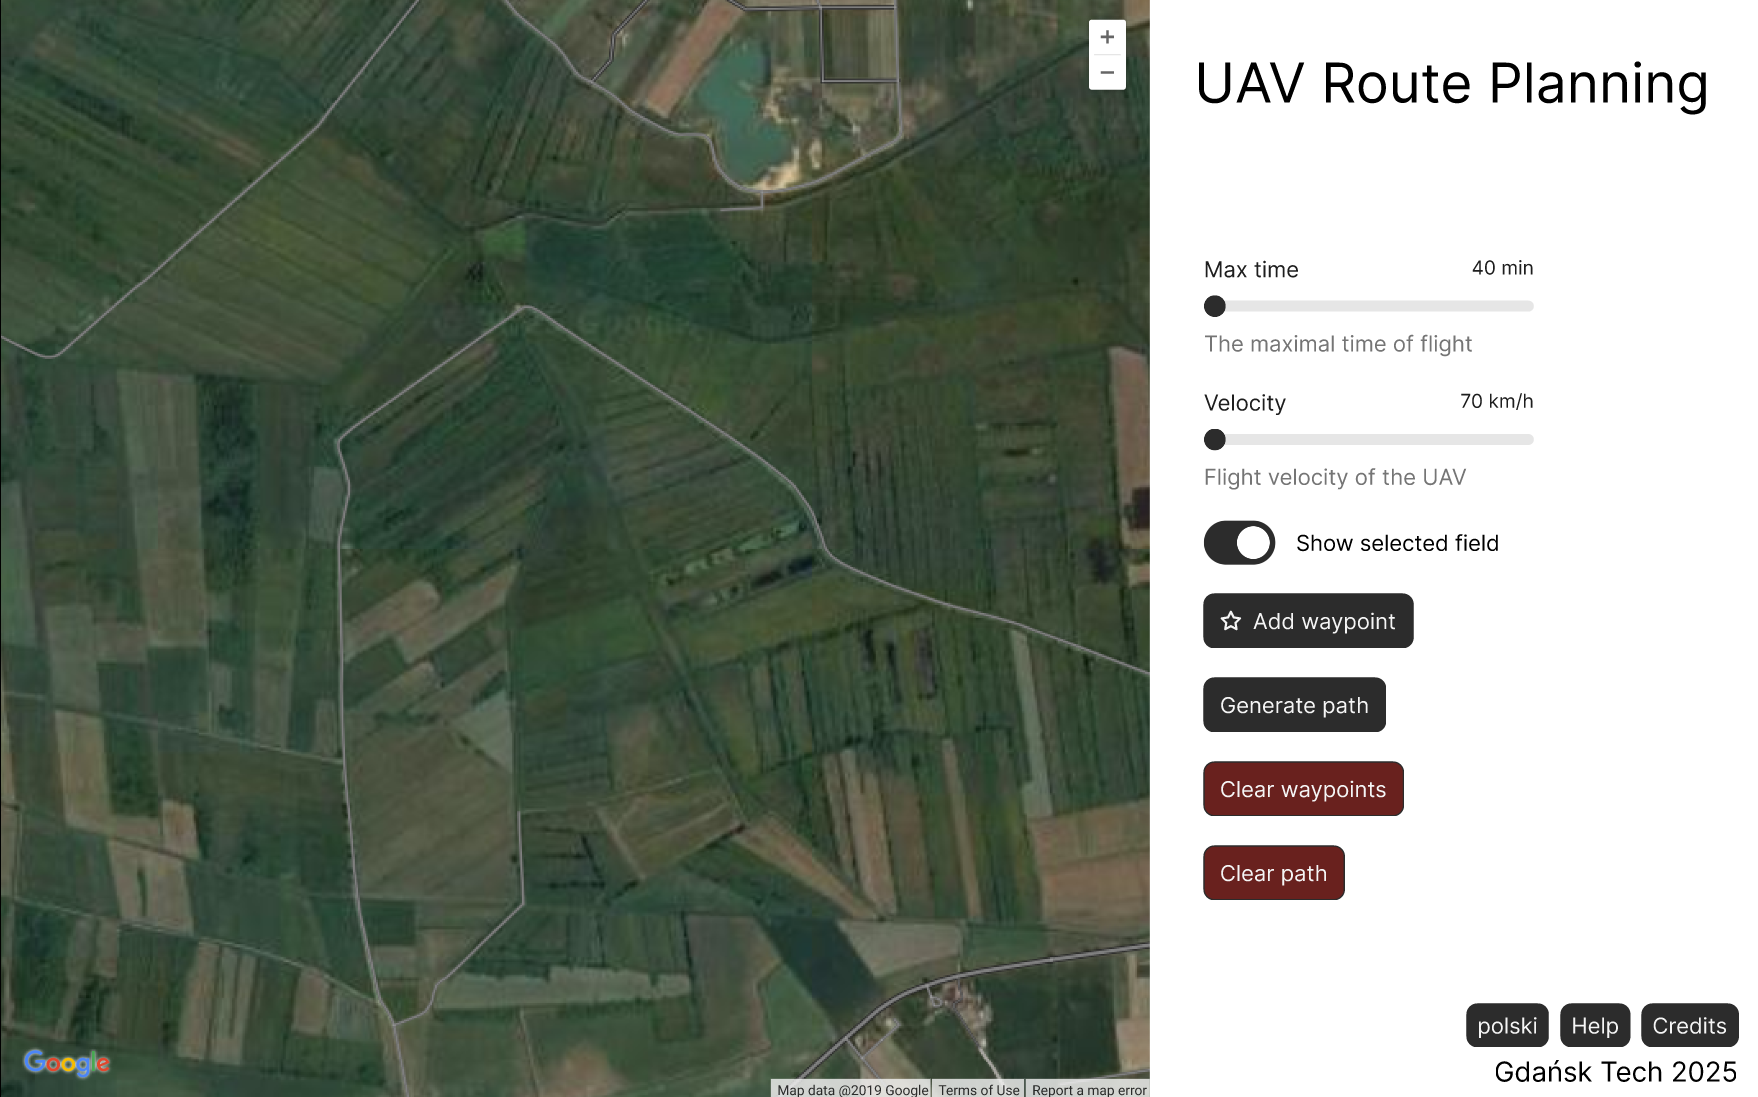
\includegraphics[width=15cm]{images/Projekt_interfejsu.png}
    \caption{Projekt interfejsu}
\end{figure}

Interfejs będzie dawał możliwość wprowadzania wymaganych do planowania trasy danych. Ponadto, po wybraniu odpowiedniej opcji będzie możliwe dodawanie punktów na mapę. Gdy użytkownik zaznaczy wszystkie punkty będzie mógł wybrać opcję planowania trasy. Jeżeli uzyskane wyniki nie będą zadowalające, możliwy będzie wybór opcji wyczyszczenia zaplanowanej trasy oraz zaznaczonych punktów na mapie. Interfejs będzie udostępniał opcję zmiany języka oraz funkcję pomocy, gdzie zostanie wyświetlony opis ułatwiający zrozumienie działania aplikacji oraz możliwe do wykonania działania.

\subsection{Wybór środowiska i implementacji}

Część aplikacji odpowiedzialna za wykrywanie krawędzi i obszarów została zaimplementowana z wykorzystaniem środowiska Colab i języka Python. Colab został wybrany z powodu łatwości w testowaniu i wizualizacji efektów osiągniętych przez zaimplementowane funkcje. Umożliwiło one łatwe porównywanie różnych parametrów rozmycia, kombinacji kanałów barw oraz różnych wartości progowania w czasie implementacji wykrywania krawędzi na obrazach.

API potrzebne do wykonywania zapytań przez interfejs użytkownika zostało zaimplementowane z wykorzystaniem środowiska PyCharm, które zostało wybrane przez zespół z powodu jego znajomości i prostoty wykorzystania. Szczególnie istotną funkcją była łatwość debugowania kodu, co w przypadku poprzedniego środowiska jest utrudnione.
Interfejs użytkownika został zaimplementowany z wykorzystaniem środowiska Visual Studio Code, które było znane członkom zespołu i jest proste w konfiguracji.

Kod projektu jest przechowywany w repozytorium GitHub, a zmiany są zapisywane w systemie kontroli wersji na bieżąco. Pozwoliło to na współpracę i dzielenie się zadaniami do wykonania oraz przeglądanie kodu i zmian na bieżąco przez każdego z członków zespołu. Dzięki komunikatom przy kolejnych wersjach zostało ułatwione utrzymanie kodu i wyłapywanie ewentualnych błędów, które pojawiły się w trakcie implementacji.

Do komunikacji w zespole był wykorzystywany Discord, na którym w razie potrzeby odbywały się spotkania zespołu w celu ustalenia planu pracy. Ponadto, w procesie wytwarzania aplikacji była wykorzystywana platforma Jira do śledzenia postępu projektu oraz tworzenia i rozdzielania zadań do wykonania, co ułatwiło dostęp do nich dla każdego z członków zespołu i uporządkowało pracę.

\subsection{Rozszerzalność aplikacji}

Aplikacja jest tworzona jako gotowy produkt umożliwiający planowanie trasy drona na wprowadzonym obszarze. Z tego powodu, prawdopodobnie nie będzie wymagała rozszerzeń w przyszłości. Mimo wszystko została ona zaprojektowana tak, że z łatwością będzie możliwe wykonanie poprawy jej funkcjonalności lub dodanie nowych.